\section{SYSTEM DESIGN AND ARCHITECTURE}
\subsection{System Overview}
\begin{figure}[h]
    \centering
    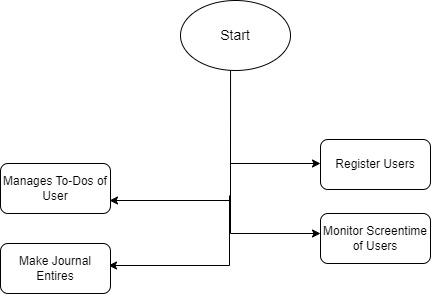
\includegraphics{system.jpg}
    \caption{Block Diagram of System}
    \label{fig:System OVerview}
\end{figure}

\newpage
\subsection{Use Case Diagram}
\begin{figure}[h]
    \centering
     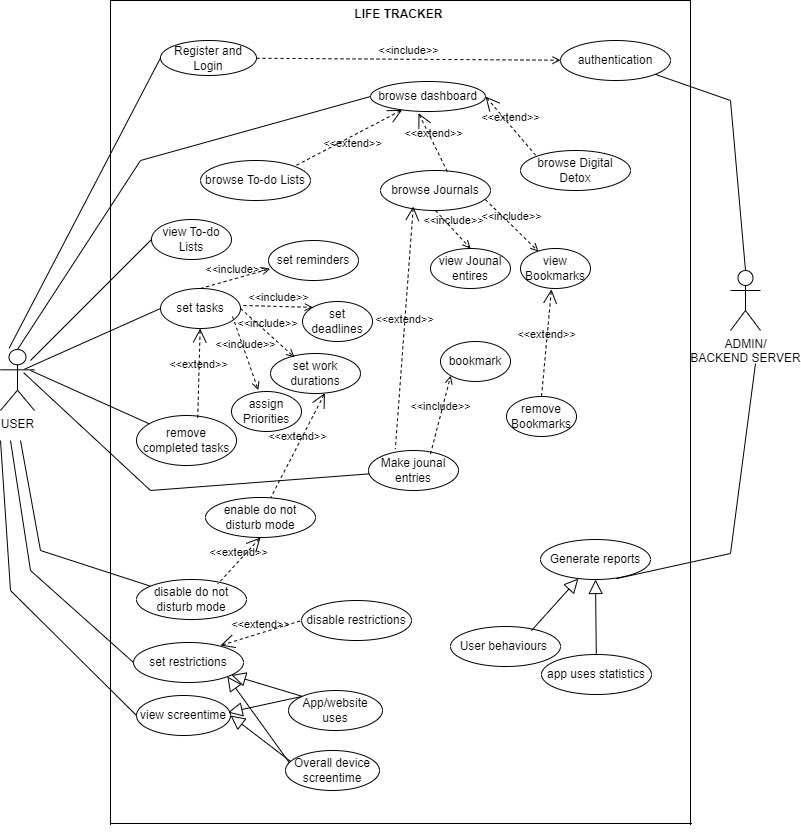
\includegraphics[width=150mm]{Use_Case.jpg}
    \caption{Use Case Diagram}
    \label{fig:Use Case Diagram}
\end{figure}

 \newpage
\subsection{Data Flow Diagram}
\begin{figure}[h]
    \centering
    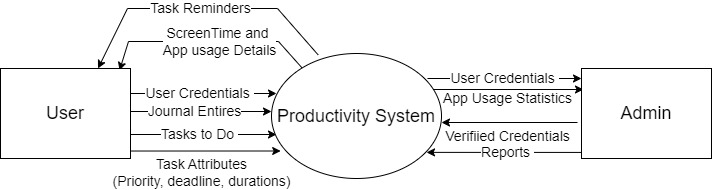
\includegraphics[width=150mm, height= 45mm]{Level0dfd.jpg}
    \caption{Level 0 DFD diagram}
    \label{fig:level 0 DFD}
\end{figure}
\vspace{0.5in}
\begin{figure}[h]
    \centering
    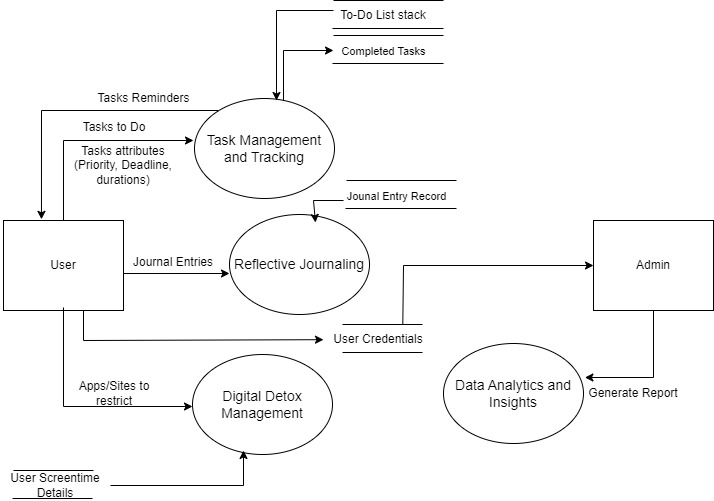
\includegraphics[width=150mm, height = 100mm]{DFDlevel1.jpg}
    \caption{Level 1 DFD diagram}
    \label{fig:level 1 DFD}
\end{figure}

\newpage
\subsection{Activity Diagram}
\begin{figure}[hbt!]
    \centering
    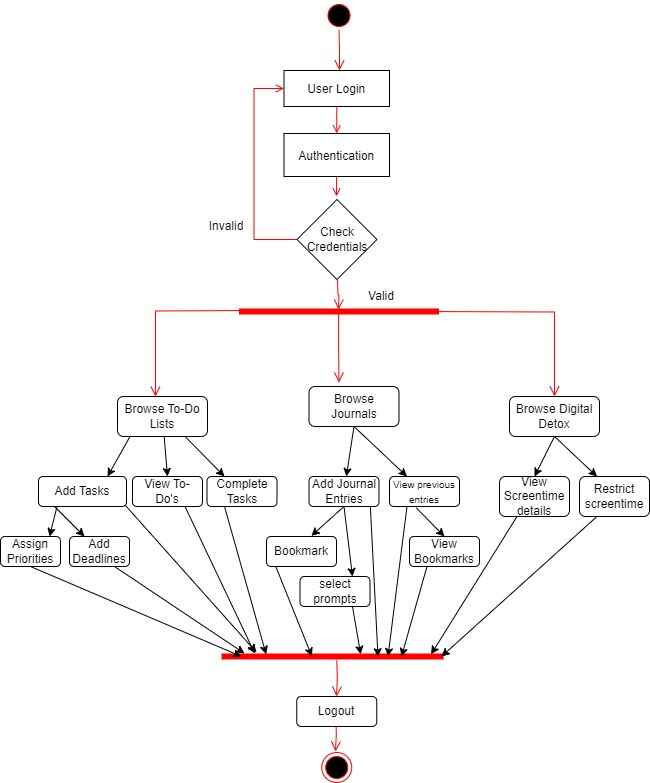
\includegraphics[width=150mm]{Activity.jpg}
    \caption{Activity Diagram}
    \label{fig:Activity Diagram }
\end{figure}

\newpage
\subsection{Sequence Diagram}
\begin{figure}[hbt!]
    \centering
     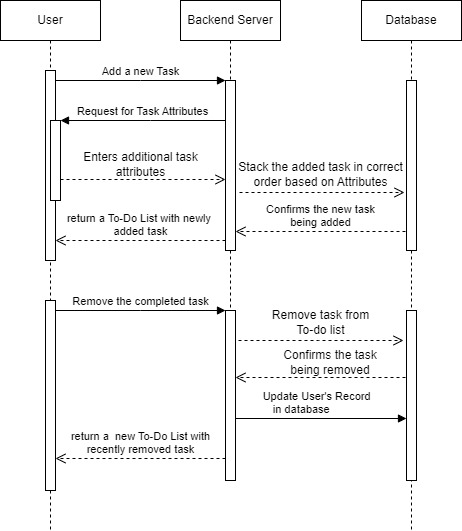
\includegraphics[width=150mm]{sequence.jpg}
    \caption{Sequence diagram for adding and removing task}
    \label{fig:Sequence Diagram}
\end{figure}
\newpage
\subsection{Class Diagram}
\begin{figure}[hbt!]
    \centering
     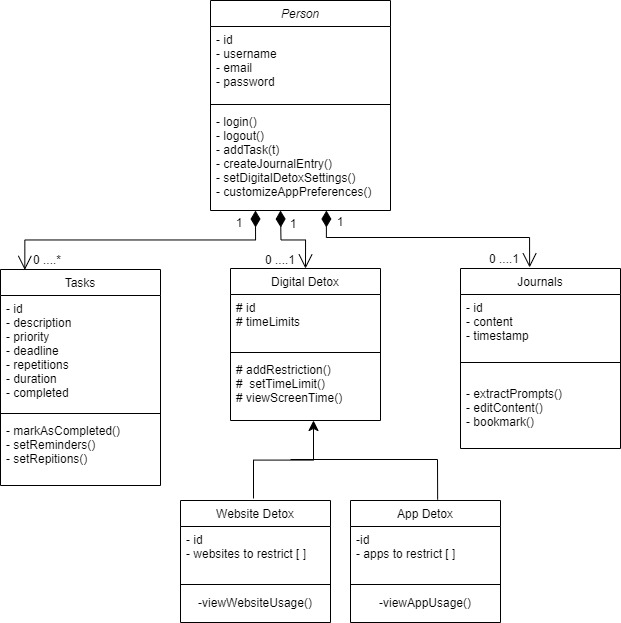
\includegraphics[width=150mm]{class.jpg}
    \caption{Class Diagram for \textit{Life Tracker} web-app }
    \label{fig:Class Diagram}
\end{figure}
